\subsection{Geographic Spread}
\label{sect:geospread}

Here we examine each cluster's geographic spread --- the closeness, in terms of
geographic distance, of members of the same cluster. As clients sharing the same
cluster are predominantly exposed to the same network resources, the geographic
spread of a cluster's clients must related to the network performance (latency)
they experience. Specifically, if a pair of clients directed
to the same network resource are physically ``far'' apart from each other, it is
likewise impossible for \emph{both} clients to simultaneously be near said
resource. In such an arrangement, the resource is either near one client and far from the other, or the
resource is equidistant from both clients. In the latter case, if the clients
are sufficiently far from each other, the resource must also far from both clients.

To calculate these geographic distances, we use coordinates for RIPE Atlas
probes --- our client machines in the context of this experiment --- obtained
from RIPE Atlas's API. RIPE acquires probe location information via manual input
from volunteers who themselves maintain Atlas probes, and, where necessary, by
autmated input from MaxMind CITE. Figure \ref{geomeans} shows the CDF of the
mean geographic distance (in kilometers) between members of a cluster, for each
cluster. Members of a cluster with a larger mean geographic distance are farther
apart form each other, on average, than are the members of a cluster with a
lower mean geographic distance. In the median case, we see an average client
distance of 509 km. We observe that for 20\% of clusters, members are over 1000
km on average. For perspective, we remind the reader that the circumference of
the world is approximately 40,075 km. 

\begin{figure}
    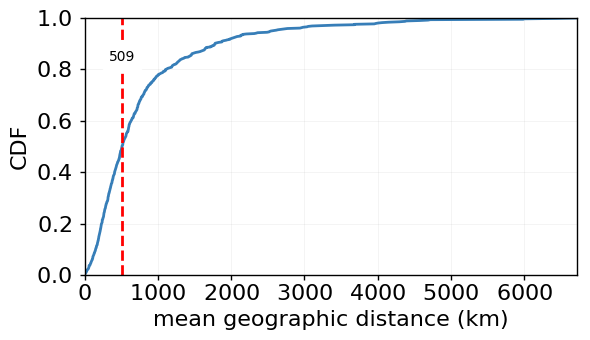
\epsfig{file=figs/geo_means.png, width=1\linewidth}
    \caption{CDF of mean geographic distance between
    cluster members. The dashed vertical line marks the median.}
    \label{geomeans}
\end{figure}

Since CNRE potentially spans many, physically distinct resources, it serves as
an \emph{aggregate} measurement and we do not attempt to pinpoint the location
of any individual resource. Instead, 

\begin{figure}
    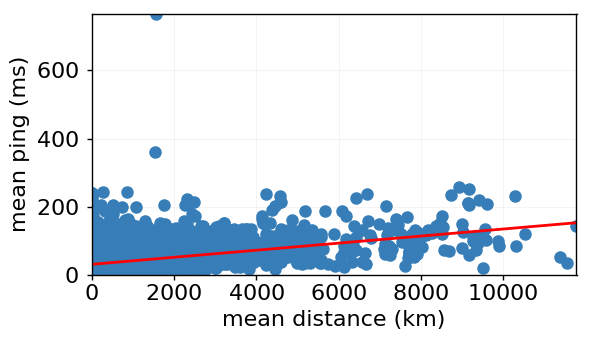
\epsfig{file=figs/geo_vs_perf.png, width=1\linewidth}
    \caption{Domain match alignment with clusters (what format?)}
    \label{geoperf}
\end{figure}
